\chapter{Génomique des procaryotes : organisation, évolution et fonctions}

Avant d'aborder la génomique comparée des procaryotes, il convient de revenir sur ce qu'est un génome procaryote. Les génomes procaryotes sont souvent décrits comme plus simple et plus facile à étudier que les génomes eucaryotes. Pourtant, sous cette simplicité apparente, il reste encore de nombreuses parts d'ombre sur l'organisation et la régulation des génomes procaryotes. Quant à la dynamique évolutive de ces génomes, nous avons vu qu'elle pose encore de nombreux problèmes aux spécialistes de la phylogénie. Enfin, les procaryotes sont toujours autant étudiés, car ce sont des réservoirs d'enzyme et processus chimique qui peuvent être utilisés dans de nombreux domaines. Des molécules et des réactions qui nous sont parfois encore inconnu et que nous sommes incapables de reproduire. Dans cette partie, je décrirais les mécanismes les plus connus et les plus répandus qui seront également des principes fondamentaux de nos hypothèses de développement méthodologique et d'analyse pangénomique. Je laisserai donc à chacun se faire une idée de la simplicité des génomes procaryotes. 

\section{Structure et organisation des génomes procaryotes}

Avant de décrire le génome, revenons rapidement sur sa définition. Le génome, c'est l'ensemble du matériel génétique, c.-à-d., des éléments qui seront hérités par les cellules de la génération suivante. Le génome, c'est aussi la structure de base qui va contenir l'ensemble des informations nécessaires au fonctionnement et à la survie de la cellule. Ces informations sont contenues dans la molécule d'ADN, ce qui nous amène à la structure primaire du génome, la séquence nucléotidique. Cette séquence est souvent circulaire chez les procaryotes et est de petite taille, quelques centaines de milliers de bases, mais certains génomes peuvent atteindre plusieurs millions de bases\footnote{En bioinformatique, on utilise l'unité base (b) ou paire de base (pb), pour mesurer la taille d'un génome. Un génome procaryote sera donc compris entre 100 kb et 10 Mb. Pour comparaison, le génome humain mesure environs 3 Gb.} (\autoref{fig:genome_size}).


\begin{figure}[htbp]
    \centering
    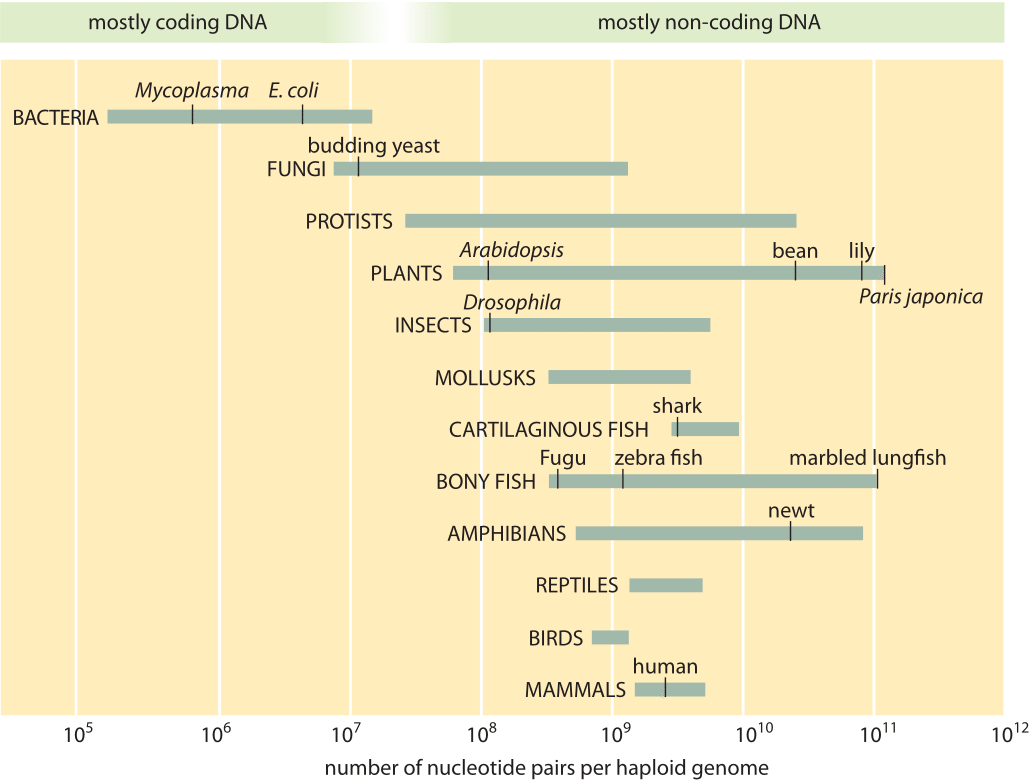
\includegraphics[width=\linewidth]{images/genome_size.png}
    \caption[Tailles des génomes pour différents groupes taxonomiques]{Variation de la taille des génomes (en paire de base) pour différents groupes taxonomiques. Copié de \cite{milo_cell_2015}}
    \label{fig:genome_size}
\end{figure}

Le génome est divisé en sous-unité que l'on appelle gène. Le gène contient l'information nécessaire pour produire une protéine qui réalisera une fonction dans la cellule (\autoref{fig:gene2prod}). Ces protéines correspondent à une chaîne d'acide aminé, que l'on peut représenter sous forme de séquence. Pour passer d'un gène à une protéine, on utilise une table de correspondance que l'on appelle code génétique où 3 nucléotides correspondent à 1 acide aminé. En moyenne, une protéine contient 300 acides aminés, ramenant la taille des gènes à environs 1 kb. Enfin, comme indiqué sur la partie haute de la \autoref{fig:genome_size}, les génomes procaryotes sont majoritairement codants, ce qui veut dire que presque tous l'ADN peut être divisé en gènes, et donc qu'il y a environs entre 100 et 10 000 gènes dans les génomes en fonction de leur taille. En mettant toutes ces informations en perspective, la petite taille des génomes procaryotes est compensé par son fort taux de gènes, ainsi, il contient l'ensemble des protéines nécessaires à la survie de la cellule. 


\begin{figure}[htbp]
    \centering
    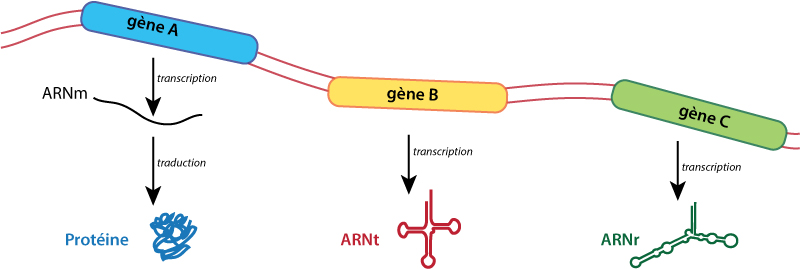
\includegraphics[width=\linewidth]{images/gene2prot.jpg}
    \caption[Produit d'un gène]{Produit d'un gène dans la cellule. Un gène est d'abord transcrit en ARN. Si l'ARN transcrit est dit messager (ARNm), il sera ensuite traduit en protéine, sinon l'ARN produit (ARNt, ARNr, miARN, ....) aura un rôle spécifique dans des processus cellulaire. Copié de RNBio, Sorbonne université. \url{https://rnbio.sorbonne-universite.fr/genetique_genotype1}}
    \label{fig:gene2prod}
\end{figure}


Dans la cellule, l'ADN ne reste pas sous cette forme primaire de séquence, il va se replier par différent mécanisme pour arriver dans une forme plus compacte qu'on appelle le chromosome (\autoref{fig:structure_dna}). L'ADN commence par se replier dans une structure secondaire, notamment la célèbre double hélice décrite par Watson, Crick et Franklin \cite{watson_molecular_1953}\footnote{Ces travaux sont souvent cités comme exemple dans la lutte pour la reconnaissance des femmes en sciences, Rosalind Franklin ayant joué un rôle essentiel, mais souvent sous-estimé dans cette découverte.}. Bien que la double hélice soit la forme la plus connue, d'autres conformations secondaires, telles que les structures en triple hélice ou en Z, ont également été identifiées, comme illustré dans la \autoref{fig:structure_dna}. L'organisation de l'ADN va au-delà de cette structure secondaire : il est ensuite soumis à des mécanismes de superenroulement induits par des enzymes spécifiques comme les topoisomérases et les gyrases. Ce superenroulement permet de réduire davantage la taille de l'ADN et de favoriser son organisation en boucles maintenues par des protéines structurales telles que HU, IHF ou H-NS \cite{williams_molecular_1997,prieto_genomic_2012}. Pour terminer des protéines appelé histones vont terminer de replier l'ADN en formant des nucléosomes, les procaryotes utilisent ces protéines pour compacter leur ADN en une structure appelée nucléoïde. Cette forme, au-delà d'optimiser l'espace dans la cellule, permet aussi de stabiliser et de protéger l'ADN, ainsi que la régulation de l’expression des gènes. Par exemple, la méthylation de l’ADN, ainsi que les modifications des protéines associées, sont des mécanismes clés de l’épigénétique. Ces processus influencent la transcription des gènes et ont des implications fonctionnelles majeures. Des études récentes ont mis en lumière le rôle de la méthylation dans la régulation de la virulence bactérienne et dans la capacité des procaryotes à coloniser leurs hôtes \cite{oliveira_bacterial_2021}, soulignant ainsi l'importance de ces mécanismes dans la survie et l’adaptation des bactéries.

\begin{figure}[htbp]
    \centering
    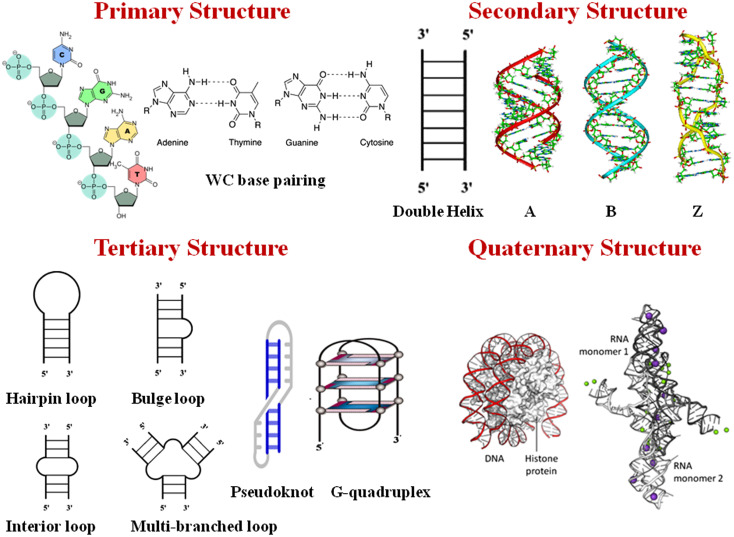
\includegraphics[width=0.8\linewidth]{images/structureDNA.jpg}
    \caption[Structure de l'ADN]{Représentation de la structure primaire, secondaire, tertiaire et quaternaire d'un acide nucléique. PDB ID : 1EQZ et 4R4V. Tiré de \cite{kumar_biomolecular_2019}}
    \label{fig:structure_dna}
\end{figure}

Un génome procaryote est donc en résumé un génome de petite taille, souvent circulaire et majoritairement codant. Il est donc essentiel de comprendre que la moindre modification dans la séquence d'ADN peut amener soit à un changement dans la séquence protéique, et donc son incapacité à fonctionner correctement, soit à l'impossibilité de produire la protéine. Une vision plus positive sera aussi d'imaginer que des changements dans la séquence d'ADN permettrons de produire une nouvelle protéine d'intérêt pour la cellule. Dans la suite, avec une vision darwinienne\footnote{Vision de l'évolution proposée par Charles Darwin, qui propose que les espèces évolue perpétuellement de façon hasardeuse et que les innovations génétiques sont ensuite maintenues ou perdues dans les populations par pression de sélection}, nous verrons par quels mécanismes la séquence d'ADN va évoluer, mais aussi comment ces évolutions seront transmises aux autres cellules procaryotes. 

\section{Dynamique évolutive des génomes : mécanismes et impacts}
\label{sec:dyn_evo}

Lorsqu'on étudie l'évolution des génomes, on s'intéresse aux changements apportés à la séquence d'ADN de la cellule : les mutations. Les mutations peuvent induire soit un gain, une perte ou une modification de la séquence génétique en fonction du mécanisme sous-jacent. Ces mécanismes sont complexes et bien différents de ceux que l'on pourrait concevoir avec une vision anthropomorphique. En effet, les cellules procaryotes ne s'accouplent pas pour produire une nouvelle cellule. Dans la nature, les procaryotes vont se multiplier par division cellulaire où une cellule mère donnera 2 cellules filles possédant le même matériel génétique que la mère, moins les possibles changements que nous décrirons dans la \autoref{sec:evo_ver}. Lorsque l'ADN est hérité de la cellule mère par la cellule fille, on va parler de \textbf{transfert vertical}. Il existe également (toujours par anthropomorphisme) une forme de sexualité des procaryotes, où 2 cellules vont échanger du matériel génétique sans qu'une nouvelle cellule ne soit créée. Dans ce cas, l'ADN est échangé entre 2 cellules dites de la même génération et on parle de \textbf{transfert horizontal} (voir \autoref{sec:evo_hz}). 

Ces mécanismes présents dans la nature sont exploités en microbiologie et en biologie cellulaire pour introduire des changements de gènes spécifiques dans une cellule et ainsi obtenir des espèces chimériques hybrident qui pourront être utilisées dans la recherche ou l'industrie \cite{baby_chromosomes_2019}. On peut aussi penser aux cellules procaryotes vivant en symbiose, voire en endosymbiose\footnote{une bactérie réside à l'intérieur d'une autre cellule (procaryote ou eucaryote)}, qui pourrait être considéré comme une étape préliminaire à une "fusion" évolutive. Ce mécanisme serait d'ailleurs à l'origine d'organites comme la mitochondrie et le chloroplaste\cite{martin_endosymbiotic_2015}. La fusion de cellules procaryotes est d'ailleurs possible et réalisée en laboratoire en enlevant leur paroi cellulaire pour obtenir des protoplastes. Les protoplastes peuvent être fusionnés grâce à des agents chimiques (comme le polyéthylène glycol) ou des chocs électriques (électrofusion) \cite{schaeffer_fusion_1976}.

\subsection{Mécanismes d'évolution par héritage}
\label{sec:evo_ver}
Les mécanismes d'évolution par héritages regroupent les processus menant à une modification du génome entre la cellule mère et la cellule fille. Théoriquement, lors de la division cellulaire, la cellule mère se divise en 2 cellules filles possédant exactement la même information génétique qu'elle. Pourtant, malgré un ensemble de mécanisme de protection et de correction de l'ADN, le génome peut différer entre les cellules mère et filles. Ce sont ces "erreurs" qui vont nous intéresser, car ce sont elles qui sont à l'origine de l'innovation et de la diversité génétique.

\subsubsection{Mutation génétique : un petit changement aux grandes conséquence}
\paragraph{\textit{Single Nucleotid Polymorphism}}

Un \textit{Single Nucleotide Polymorphism} (SNP) est un mécanisme d'évolution qui induit une modification de la séquence par la transformation d'un nucléotide en un autre. Étant donné que le code génétique est dégénéré\footnote{Un acide aminé peut être codé par plusieurs codons différents.}, la mutation peut ne pas avoir d'impact sur la séquence de la protéine, on dit que la mutation est silencieuse ou même sens. Si la modification change la séquence protéique, dans ce cas, on parle de mutation faux-sens. Enfin, Une mutation est qualifiée de non-sens lorsqu'elle affecte un point clé de la séquence protéique, comme le site actif ou un codon STOP, entraînant une perte de fonction de la protéine, ou lorsqu'elle introduit prématurément un codon STOP dans la séquence.

\paragraph{Indels: insertion, délétion et pseudogènes}

Un indel correspond à l'insertion (In) ou la délétion (del)\footnote{On regroupe l'insertion et la délétion, car sans une analyse phylogénétique, il est impossible de les différencier par comparaison de séquence.} d'un ou plusieurs nucléotides dans la séquence d'un gène. 

Lorsque la taille de l'indel est un multiple de 3 (insertion ou délétion d'un codon), la séquence protéique peut soit être allongé ou raccourci d'un acide aminé, soit coupé de façon précoce si le codon est un codon STOP.

Si la taille de l'indel n'est pas un multiple de 3, il y aura un décalage du cadre de lecture ou \textit{frameshift}. Ce décalage va induire un changement de tous les acides aminés de l'indel à la fin du gène, provoquant avec lui un changement dans la fonction de la protéine ou une inactivation de la fonction. La partie du gène qui n'est pas décalé est alors considéré comme un fragment du gène initial, il est alors qualifié de pseudogène. À nouveau, cette mutation peut être délétère pour la cellule. 

Les indels vont donc transformer la séquence protéique traduite, pouvant nuire à la fonction de cette dernière et être délétère pour l'organisme. Pour éviter les problèmes liés au \textit{frameshift}, il a été montré qu'il existe un fort taux de codon STOP hors du cadre de lecture \cite{tse_natural_2010}. Cette adaptation permettrait de limiter la traduction des protéines mutante et d'ainsi limiter le coût énergétique pour la cellule. Il a aussi été montré que les \textit{frameshift} pourrait être à l'origine d'un réservoir d'adaptation à l'environnement \cite{koch_catastrophe_2004}. Lors d'un changement dans l'environnement créant une nouvelle pression de sélection, un \textit{frameshift} pourrait améliorer le fitness de certains organismes. Une fois que l'élément perturbateur de l'environnement disparait, un nouveau frameshift ramènerait le cadre de lecture à sa place d'origine. Ce mécanisme, en accord avec la petite taille des génomes, aurait l'intérêt de ne pas perdre des gènes d'adaptation à l'environnement, même s'ils ne sont nécessaires que ponctuellement.

\subsubsection{Réarrangement génomique : un moteur de l'évolution}
\paragraph{Réarrangement}
\paragraph{Recombinaison}
\paragraph{Duplication}

\subsection{Mécanismes d'évolution intragénérationnelle}
\label{sec:evo_hz}

\subsubsection{Conjugaison : la sexualité des procaryotes}

\subsubsection{Transformation : recycler l'ADN environnant}

\subsubsection{Transduction : un sacrifice pour le bien commun}

\subsection{Interprétation des évolutions : l'homologie et ses déclinaisons}


\section{Du génome aux processus cellulaires : exploration fonctionnelle}

\subsection{Gènes et fonctions}

\subsection{Îlots génomiques}
